\section{Methodology}\label{sec:methodology}
As part of our goal to evaluate the performance of each of the components in the pipeline, the first step was to create a replica of the original pipeline described by \citeauthor{cleggRecalibrationMarsScience2017}
Since we did not have access to the original source code implementing the pipeline, we have replicated it at accurately as we could based on the available information.
However, not all details were included in this report, so we have had to make some assumptions, which we detail here.
In addition, some aspects of the pipeline rely on qualitative assessments made by the original authors --- something we cannot do because we are not domain experts.
Consequently, our pipeline is not identical to the original, but we have strived to make it as close as possible.

This section is dedicated to describing the methodology of our pipeline, how it differs from the original, and which design choices we have made and why.
Furthermore, we delve into the experiments we have conducted to evaluate the performance of our pipeline such that we can identify the components that contribute the most to the overall error.

\subsection{Data Shape and Preprocessing}
Part of the data preprocessing is shared between the PLS1-SM and ICA phases of the pipeline.
However, each phase also has its own preprocessing steps, which are described in sections \ref{sec:pls1_data_preprocessing} and \ref{sec:ica_data_preprocessing} respectively.
This section describes the preprocessing steps that are common to both phases.

For each target, the data is split into five datasets, one for each location on the sample that was shot at by the laser.
Each dataset contains CCS data stored in a \texttt{.csv} file, which is read into a Pandas dataframe\cite{pandas} using the \texttt{read\_csv} function.
Because the CCS data includes several lines of header information, we skip these lines using the \texttt{skiprows} parameter.
We then remove the first five shots from the data similarly to \citeauthor{cleggRecalibrationMarsScience2017}.
These first five shots are typically contaminated by dust that covers the target before being removed by the laser-produced shock waves.
Finally, we mask the edges of the spectral regions of the data to eliminate increased noise, especially in areas where small intensity changes lead to large variations in the calibrated signal.
The masked regions, which do not contain unique major element diagnostic peaks, are excluded to enhance the accuracy and reliability of the quantitative analysis.
These regions are defined in \citeauthor{cleggRecalibrationMarsScience2017} 40.811 - 246.635, 338.457 - 340.797, 382.138 - 387.859, 473.184 - 492.427, and 849 - 905.574 nm.
An illustration of these masked regions can be seen in figure \ref{fig:masked_regions}.

\begin{itemize}
	\item The code starts by setting up criteria to exclude specific columns (like "wave", "mean", and "median") from certain operations and identifies the first five shots in the data.
	\item For each sample dataset, the code cleans the column names by stripping whitespace and removing specific characters. It also ensures the consistency of wavelength data across different datasets.
	\item The code removes certain predefined columns and re-inserts wavelength data to maintain its structure in the dataframe.
	\item If enabled, the code computes the average of certain columns (related to shots) and adds this average back into the dataset, while removing the original shot columns.
	\item Each processed dataset is compiled into a list, which is then returned for further use.
	\item Masking is performed on the data to remove the spectral-range edges.
\end{itemize}


\subsection{PLS1-SM}
This section describes the PLS1-SM aspect of the pipeline.

\subsubsection{Data Preprocessing}\label{sec:pls1_data_preprocessing}

\subsubsection{Outlier Removal with Mahalanobis Distance and Chi-Squared Test}
% General programming language differences and implementation details
% Differences in outlier detection (automatic/quantitative vs manual/qualitative)
% Missing information about how three of the oxides are weighted in MOC result
% No manual cross validation in PLS
% Holdout split 80/20
% No inverse IRF weighing weighting in ICA
% Missing information about outlier removal in ICA - therefore we decided to not do it
% Missing information about how ICA uses each of the five datasets for each target
% How we do regression in ICA (since there are not enough details about it in the papers)

As mentioned in section \ref{sec:outlier_removal}, if the Mahalanobis distances can be shown to follow a chi-squared distribution, then the chi-squared test can be used to determine whether a sample is an outlier.
Since we do not have the expertise to make a qualitative assessment of the outliers, we have instead decided to use this property of the Mahalanobis distances to automatically detect outliers.
This works by computing the Mahalanobis distance for each data point in the training set, followed by a comparison of these distances against a chi-squared distribution.
A data point is classified as an outlier if its Mahalanobis distance corresponds to a chi-squared statistic that exceeds the critical value of the chi-squared distribution, which is determined by the specified degrees of freedom $df$.
The critical value is determined by the significance level $\alpha$ and the number of degrees of freedom $df$.
Since we have leverage and spectral residuals as our two dimensions, we have $df = 2$, because the number of dimensions is equal to the number of degrees of freedom\cite{aggarwal_outlier_2017}.
% TODO: Describe why we chose the degrees of freedom we did, and how we used this chi-squared test to determine outliers.

The outlier removal process is done iteratively because of the phenomenon described in \citeauthor{cleggRecalibrationMarsScience2017} where removing outliers can cause new outliers to appear.
The process is as follows:
\begin{enumerate}
    \item Compute the Mahalanobis distances for each sample in the training set.
    \item Determine chi-squared statistics for these distances.
    \item Eliminate outliers exceeding the chi-squared critical value.
    \item Train a new model on the remaining samples.
    \item Repeat until model no longer improves as measured by the RMSE.
\end{enumerate}


It should be noted that our outlier removal process is conservative to avoid removing too many samples and as such, we have set our significance level $\alpha$ to 0.975.
This means that we are willing to accept a 2.5\% chance of falsely removing a sample that is not an outlier.

\subsection{ICA}
The ICA phase in our pipeline, which can be seen in figure \ref{fig:ica_data}, represents a mostly faithful replication of the original, with a few considered adjustments and exclusions due to incomplete details about the original implementation.
In this section, we delve into these differences and the rationale behind our choices, maintaining a strong alignment with the overall methodology of the original pipeline.

\subsubsection{Data Preprocessing}\label{sec:ica_data_preprocessing}
Similar to the original pipeline, we have used the samples from the ChemCam calibration dataset.
Before performing ICA, we have to preprocess this data, which is illustrated in figure \ref{fig:ica_data}.
As in section \ref{sec:...}, we start by masking the data such that the emission lines in the spectral-range edges are removed. %TODO: update reference when PLS section is done
Then we normalize the data --- once using Norm1 and once using Norm3.
This gives us two datasets with normalized data.
Both of these datasets are then used for ICA separately because, as \citeauthor{cleggRecalibrationMarsScience2017} found, some of the oxides are better modeled with data normalized using Norm1, while others are better modeled with data normalized using Norm3.
The independent components from each of these two datasets are saved to a file and used for regression later.
These steps are identical to the original pipeline described by \citeauthor{cleggRecalibrationMarsScience2017}

\begin{figure}
	\centering
	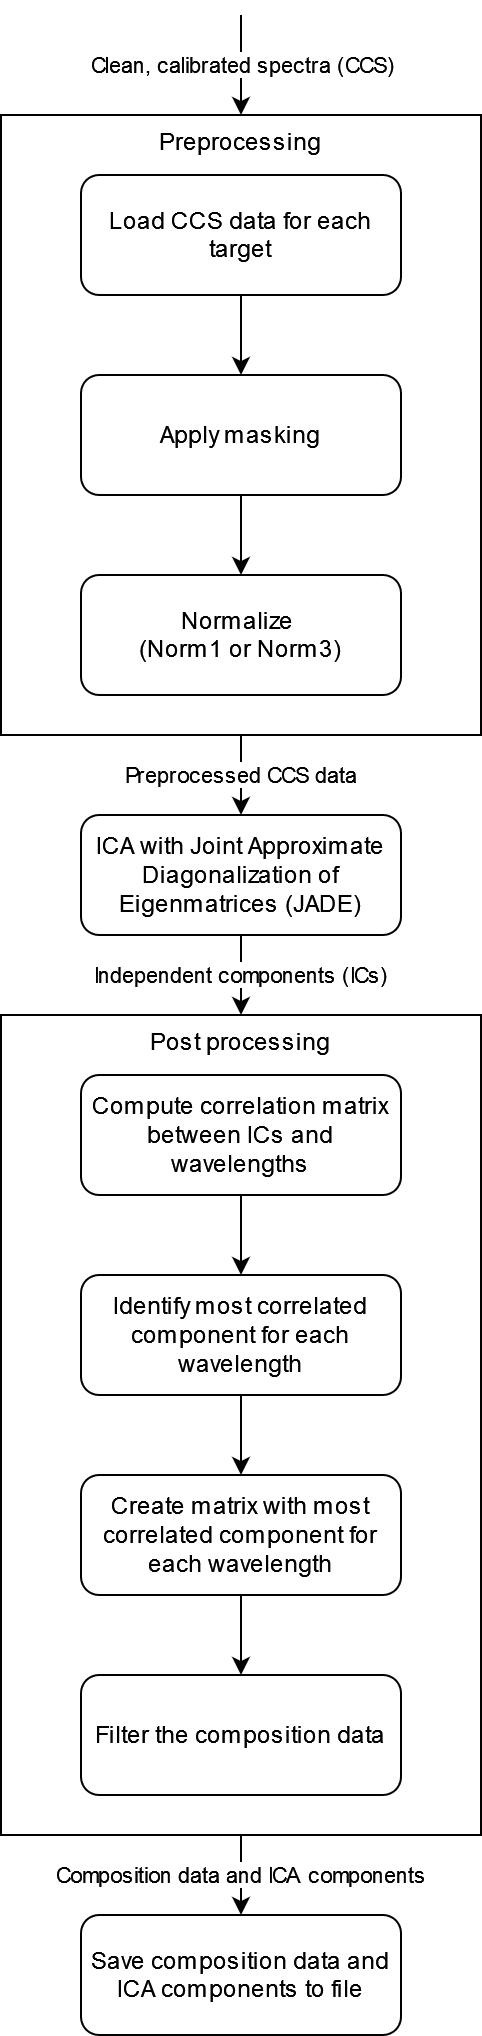
\includegraphics[width=0.2675\textwidth]{images/ica_data.png}
	\caption{The ICA phase in our recreation of the pipeline.}
	\label{fig:ica_data}
\end{figure}

However, we do not weigh by the inverse of the instrument response function (IRF) as mentioned in \citeauthor{cleggRecalibrationMarsScience2017} before normalizing.
The purpose of the IRF is to calibrate the measured signal to physical units since different pixels have different sensitivities.
For example, pixels located at the edge of a CCS usually exhibit lower sensitivity compared to those at the center, and the optics vary in their reflective and absorptive properties at different wavelengths.
One argument for inverting the IRF is that it introduces more noise in areas of interest on the spectrum by multiplying with a high value as part of the conversion to physical units.
However, the issue with this method is that it discards the alignment between the spectral data collected by the instrument in Los Alamos and the spectral data collected by the instrument on Mars.
If the same instrument were used for all analyses, one could argue that the IRF (apart from the inverse square law correction) part is irrelevant, but that is not the case here; there are two different instruments --- one in Los Alamos and one on Mars.
Based on these considerations, we have decided to not weigh by the inverse of the IRF.

In addition, because \citeauthor{cleggRecalibrationMarsScience2017} does not mention how each of the five location datasets are used for each target, we have decided to only use one for each target.
This likely does not produce as accurate results as using all five location datasets would, since we do not get a full representation of the sample that was shot at by the laser, instead only getting a partial representation from a single location.
Nevertheless, to avoid deviating significantly from \citeauthor{cleggRecalibrationMarsScience2017}'s methodology or making unfounded assumptions about their data processing, we have opted for this more conservative approach.
Our goal is to test each of the components of the pipeline individually rather than trying to reproduce the results to absolute perfection.

Similarly, in our replica of the pipeline, we have not incorporated outlier detection in the ICA part of the pipeline primarily because \citeauthor{cleggRecalibrationMarsScience2017} does not describe their implementation sufficiently enough for replication without unsubstantiated assumptions.
They mention the use of Median Absolute Deviation for this purpose, but the specifics of their approach remain unclear.
Our decision to omit outlier detection in the ICA phase of our pipeline is also influenced by a preference for retaining a more comprehensive dataset, despite the potential inclusion of outliers.
Further supporting this decision is input from one of the original authors involved in the ChemCam project.
This author highlighted the extensive efforts invested in developing the ChemCam calibration dataset, suggesting a low presence of significant outliers.
While it would be ideal to include outlier detection in the ICA phase to ensure alignment with the original pipeline, implementing it based on substantial assumptions would be counterproductive, potentially compromising the integrity of our analysis.

After examining the results in section \ref{sec:results}, we will discuss the implications of these design choices in section \ref{sec:discussion}.

\subsection{Joint Approximate Diagonalization of Eigenmatrices (JADE) and Regression}
After preprocessing the data, we are ready to perform ICA.
This is done using the Joint Approximate Diagonalization of Eigenmatrices (JADE) algorithm, which is used to calculate the mixing matrix.
This mixing matrix is an $N \times M$ matrix, where $N$ is the number of samples and $M$ is the number of independent components.
By taking the product of the mixing matrix and the normalized data, we get the estimated sources.
This new matrix is an $M \times P$ matrix, where $M$ is the number of independent components, and $P$ is the number of wavelengths.

After performing ICA, we post-process by computing the correlation between the independent components and the wavelengths.
Using this, we can identify which wavelengths are associated with which independent components by computing the maximum correlation for each wavelength.
This gives us a matrix of ICA scores that we then use for regression.

\begin{figure}
	\centering
	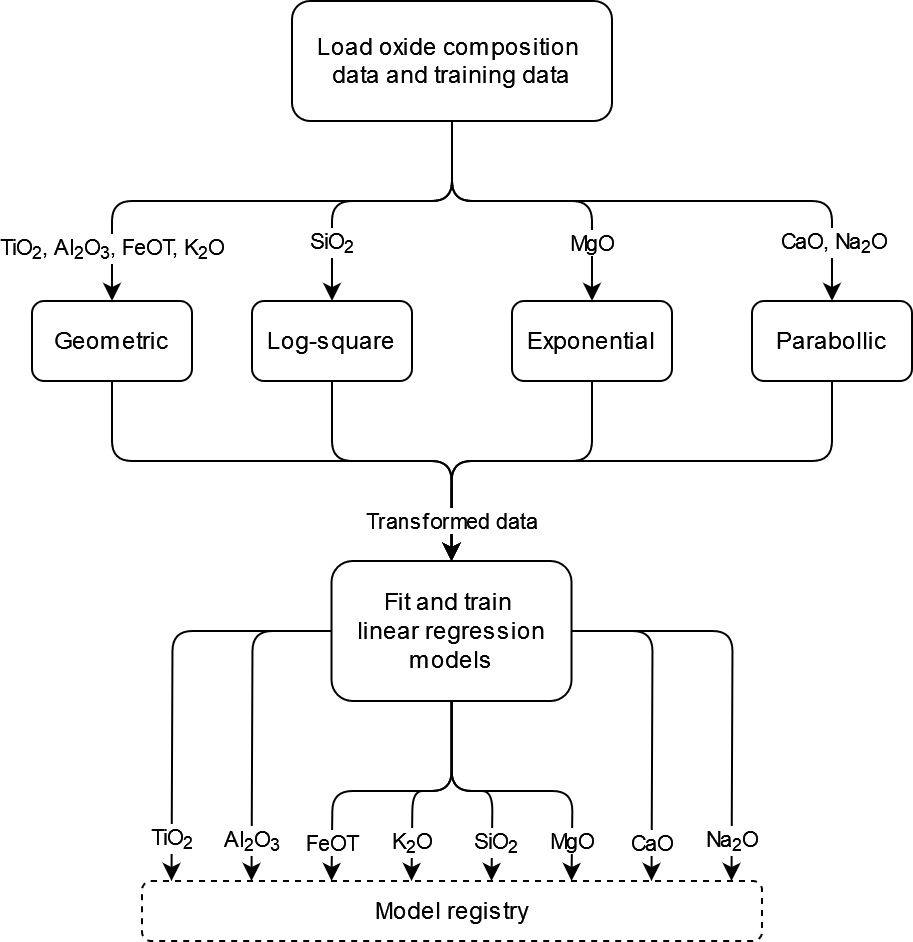
\includegraphics[width=0.45\textwidth]{images/ica_regression.png}
	\caption{Regression in the ICA phase of our recreation of the pipeline.}
	\label{fig:ica_regression}
\end{figure}

The regression process is illustrated in figure \ref{fig:ica_regression}.
Since we are implementing this recreation in Python, a different programming language than the original pipeline, we cannot use the same libraries for regression.
We use the \texttt{LinearRegression} class from the \texttt{scikit-learn} library\cite{scikit-learn}.
However, \citeauthor{cleggRecalibrationMarsScience2017} mentions performing four more types of regression in addition to linear regression, namely parabolic, exponential, geometric and logsquare.
For each oxide, they used the type of regression and normalization that produced the best results.

% TODO: Move this table to the results section and embed our own results in it as well to show the baseline results compared to the original results.
% This can be seen in table \ref{tab:regression_types}, which is taken from \citeauthor{cleggRecalibrationMarsScience2017}.

% \begin{table}[h]
% \centering
% \begin{tabular*}{\columnwidth}{@{\extracolsep{\fill}}lccc}
% \toprule

% Element & Norm & Law type    & RMS \\ \midrule
% Si      & 1    & Logsqaure   & 6.7 \\
% Ti      & 3    & Geometric   & 0.6 \\
% Al      & 3    & Geometric   & 4.4 \\
% Fe      & 1    & Geometric   & 2.2 \\
% Mg      & 1    & Exponential & 3.0 \\
% Ca      & 1    & Parabolic   & 1.0 \\
% Na      & 3    & Parabolic   & 0.6 \\
% K       & 3    & Geometric   & 0.4 \\
% \bottomrule
% \end{tabular*}
% \caption{The summary of each ICA model characteristics from \citeauthor{cleggRecalibrationMarsScience2017}.}
% \label{tab:regression_types}
% \end{table}

% TODO: Update/rewrite this to reflect the new curve-fit implementation.
% Because \texttt{scikit-learn} does not support these types of regression, we instead opted to transform the data to fit the linear regression model.
% For example, to perform exponential regression, we take the natural logarithm of the data, perform linear regression, and then take the exponential of the result.
% This is done for each of the four types of regression mentioned above.
% The code for this can be seen in listing \ref{lst:data_transformation}.

% \begin{lstlisting}[
% 	language=Python,
% 	caption={The code for transforming the data to fit the linear regression model.},
% 	label={lst:data_transformation}
% 	]
% if model_name == "Log-square":
% 	X_train = np.log(X_train**2)
% 	X_test = np.log(X_test**2)
% elif model_name == "Exponential":
% 	X_train = np.log(X_train)
% 	X_test = np.log(X_test)
% elif model_name == "Geometric":
% 	X_train = np.sqrt(X_train)
% 	X_test = np.sqrt(X_test)
% elif model_name == "Parabolic":
% 	X_train = np.column_stack((X_train, X_train**2))
% 	X_test = np.column_stack((X_test, X_test**2))
% \end{lstlisting}

In summary, we have created a replica of the ICA phase of the pipeline with strategic adaptations to accommodate the differences in programming language and the missing or unclear information about the original implementation.

\subsection{MOC}
As mentioned in section \ref{sec:moc}, the result of the PLS1-SM and ICA are combined to produce the final MOC model.
This is done by taking a weighted average of the two models, where the weights are determined based on the fact that one technique is be better suited for certain elements than the other.
These weights can be seen in table \ref{tab:weighted_sum_oxide}.
Note that the weights for Ti, Mg and Ca have been set to 50/50 since \citeauthor{cleggRecalibrationMarsScience2017} does not mention the weights they used for these elements.

\begin{table}[h]
\centering
\begin{tabular*}{\columnwidth}{@{\extracolsep{\fill}}lcc}
\toprule
Element  & PLS1-SM (\%) & ICA (\%) \\ \midrule
Al       & 75           & 25      \\
Fe       & 75           & 25      \\
Si       & 50           & 50      \\
Na       & 40           & 60      \\
K2       & 25           & 75      \\
Ti*      & 50           & 50      \\
Mg*      & 50           & 50      \\
Ca*      & 50           & 50      \\
\bottomrule
\end{tabular*}
\caption{Weighted Sum of Oxide Percentages. Elements marked with an asterisk (*) have been set to 50/50 as they are unspecified in \citeauthor{cleggRecalibrationMarsScience2017}}
\label{tab:weighted_sum_oxide}
\end{table}



% \textit{Recreate the current model. Reproduce the results of the original papers. Investigate the limitations of the model and propose improvements.}


% \section{Framework for at kunne analysere data}
% Hold out split 80/20 - har lavet cross validation på træningssæt

% \section{Outlier removal}
% \section{Ikke lavet outlier removal i ICA}
% \section{Har ikke lavet inverse IRF}
% \section{Ved ikke hvordan 3 oxider er vægtet i MOC}
% This section explains how the research was conducted.
% - Purpose: To detail the experiments, algorithms, and data sets used, enabling reproducibility.
% - Subsections: Can include Experiment Design, Algorithm Descriptions, Data Sources, and Evaluation Metrics.
% - Best Practices: Be explicit about every aspect of your methodology, including any limitations.

% Research Design
% - Overall plan for conducting the study
% Data Collection Methods
% - Description of how data was collected
% Algorithms and Models
% - Detailed explanation of algorithms, models, or frameworks used
% Evaluation Criteria
% - Metrics used to evaluate the outcomes